\documentclass[12pt]{article}

\usepackage{amsmath}
\usepackage{amssymb}
\usepackage{amsfonts}
\usepackage{amsthm}
\usepackage{graphicx}
\usepackage{hyperref}

\title{State of Quanutm Machine Learning:\\
\large Analysis of Quantum Neural Networks\\ 
and Linear Regression}
\author{Ryan Dougherty}
\date{\today}

\begin{document}

\maketitle

\section*{Introduction}
Quantum machine learning (QML) is a new approach to typical machine learning algorithms that takes advantage of superposition and entanglement to provide upwards of exponential speedup. QML is still in very early stages of its development. The goal of this paper is to discuss the current state of QML and its potential for the future. It will also go over the upsides as well as the downsides of QML. I will go over the classical approach to machine learning and how QML differs from it. I will also go over some examples of QML in action and how it is being used today. Finally, I will conclude with my personal thoughts on the subject and provide some recommendations for further reading.

\section*{Classical Approach To Machine Learning}
Classical approaches to machine learning are based on the idea of a using a generalized function that maps a set of fit inputs to outputs. The output can then be used to make predictions about new inputs. The overarching goal of machine learning is to find the best function that accurately guesses the output for a given input with a desired accuracy. There are many approaches to machine learning. In this paper I will go over two specific approaches: 
\begin{itemize}
\item \textbf{Neural Networks}: Neural networks work similar to neurons in the human brain. They are made up of layers of nodes that are connected to each other. Each node has a weight that is multiplied by the input and then added to the sum of the other nodes. The sum is then passed through an activation function to produce a desired output. The weights are then adjusted to minimize the error between the output and the desired output. Neural networks are often used in natural language processing and image recognition.
\item \textbf{Linear Regression}: Linear regression is a supervised learning algorithm that is used to predict a continuous output. Supervised learning is when your algorithm is attempting to find a specific output based on its given input; it will continually refine its decission and prediction process to ensure its outputs match their desired results. Linear regression is based on the idea of a linear function that maps the input to the output. The goal is to find the best linear function that accurately predicts the output for a given input. Linear regression is mainly create prediction models, for example, predicting future stock and housing prices.
% \item \textbf{Logistic Regression}: Logistic regression is a supervised learning algorithm that is used to predict a binary output. It is based on the idea of a logistic function that maps the input to a desired output. The goal is to find the best logistic function that accurately predicts the output for a given input. It can be used for classifcation; For example, categorizing important emails versus spam emails.
% \item \textbf{Decision Trees}: Decision trees are another supervised learning algorithm. They are used to predict a categorical output. They are based on the idea of a tree structure where each node represents a feature and each branch represents a possible outcome. The goal is to find the best tree structure that accurately predicts the output for a given input. Decision trees are often used in predicting the best medical diagnosis given a patient's symptoms.
% \item \textbf{Clustering}: Clustering is an unsupervised learning algorithm. Unsupervised learning is used when the data does not have a desired output. The goal is instead to find patterns in the input data and categorize it accordingly. For example, clustering can be used to find similar customers based on their purchase history.
\end{itemize}

\section*{Quantum Approach}
Now that I've gone over the classical approach to machine learning, let's discuss the quantum approach to machine learning. In a nutshell, QML algorithms are developed by projecting their classical counterparts into a hilbert space representable by quantum states. This allows for the use of quantum superposition and entanglement to provide significant speedup not possible on classical computers.

\begin{figure}[h]
\centering
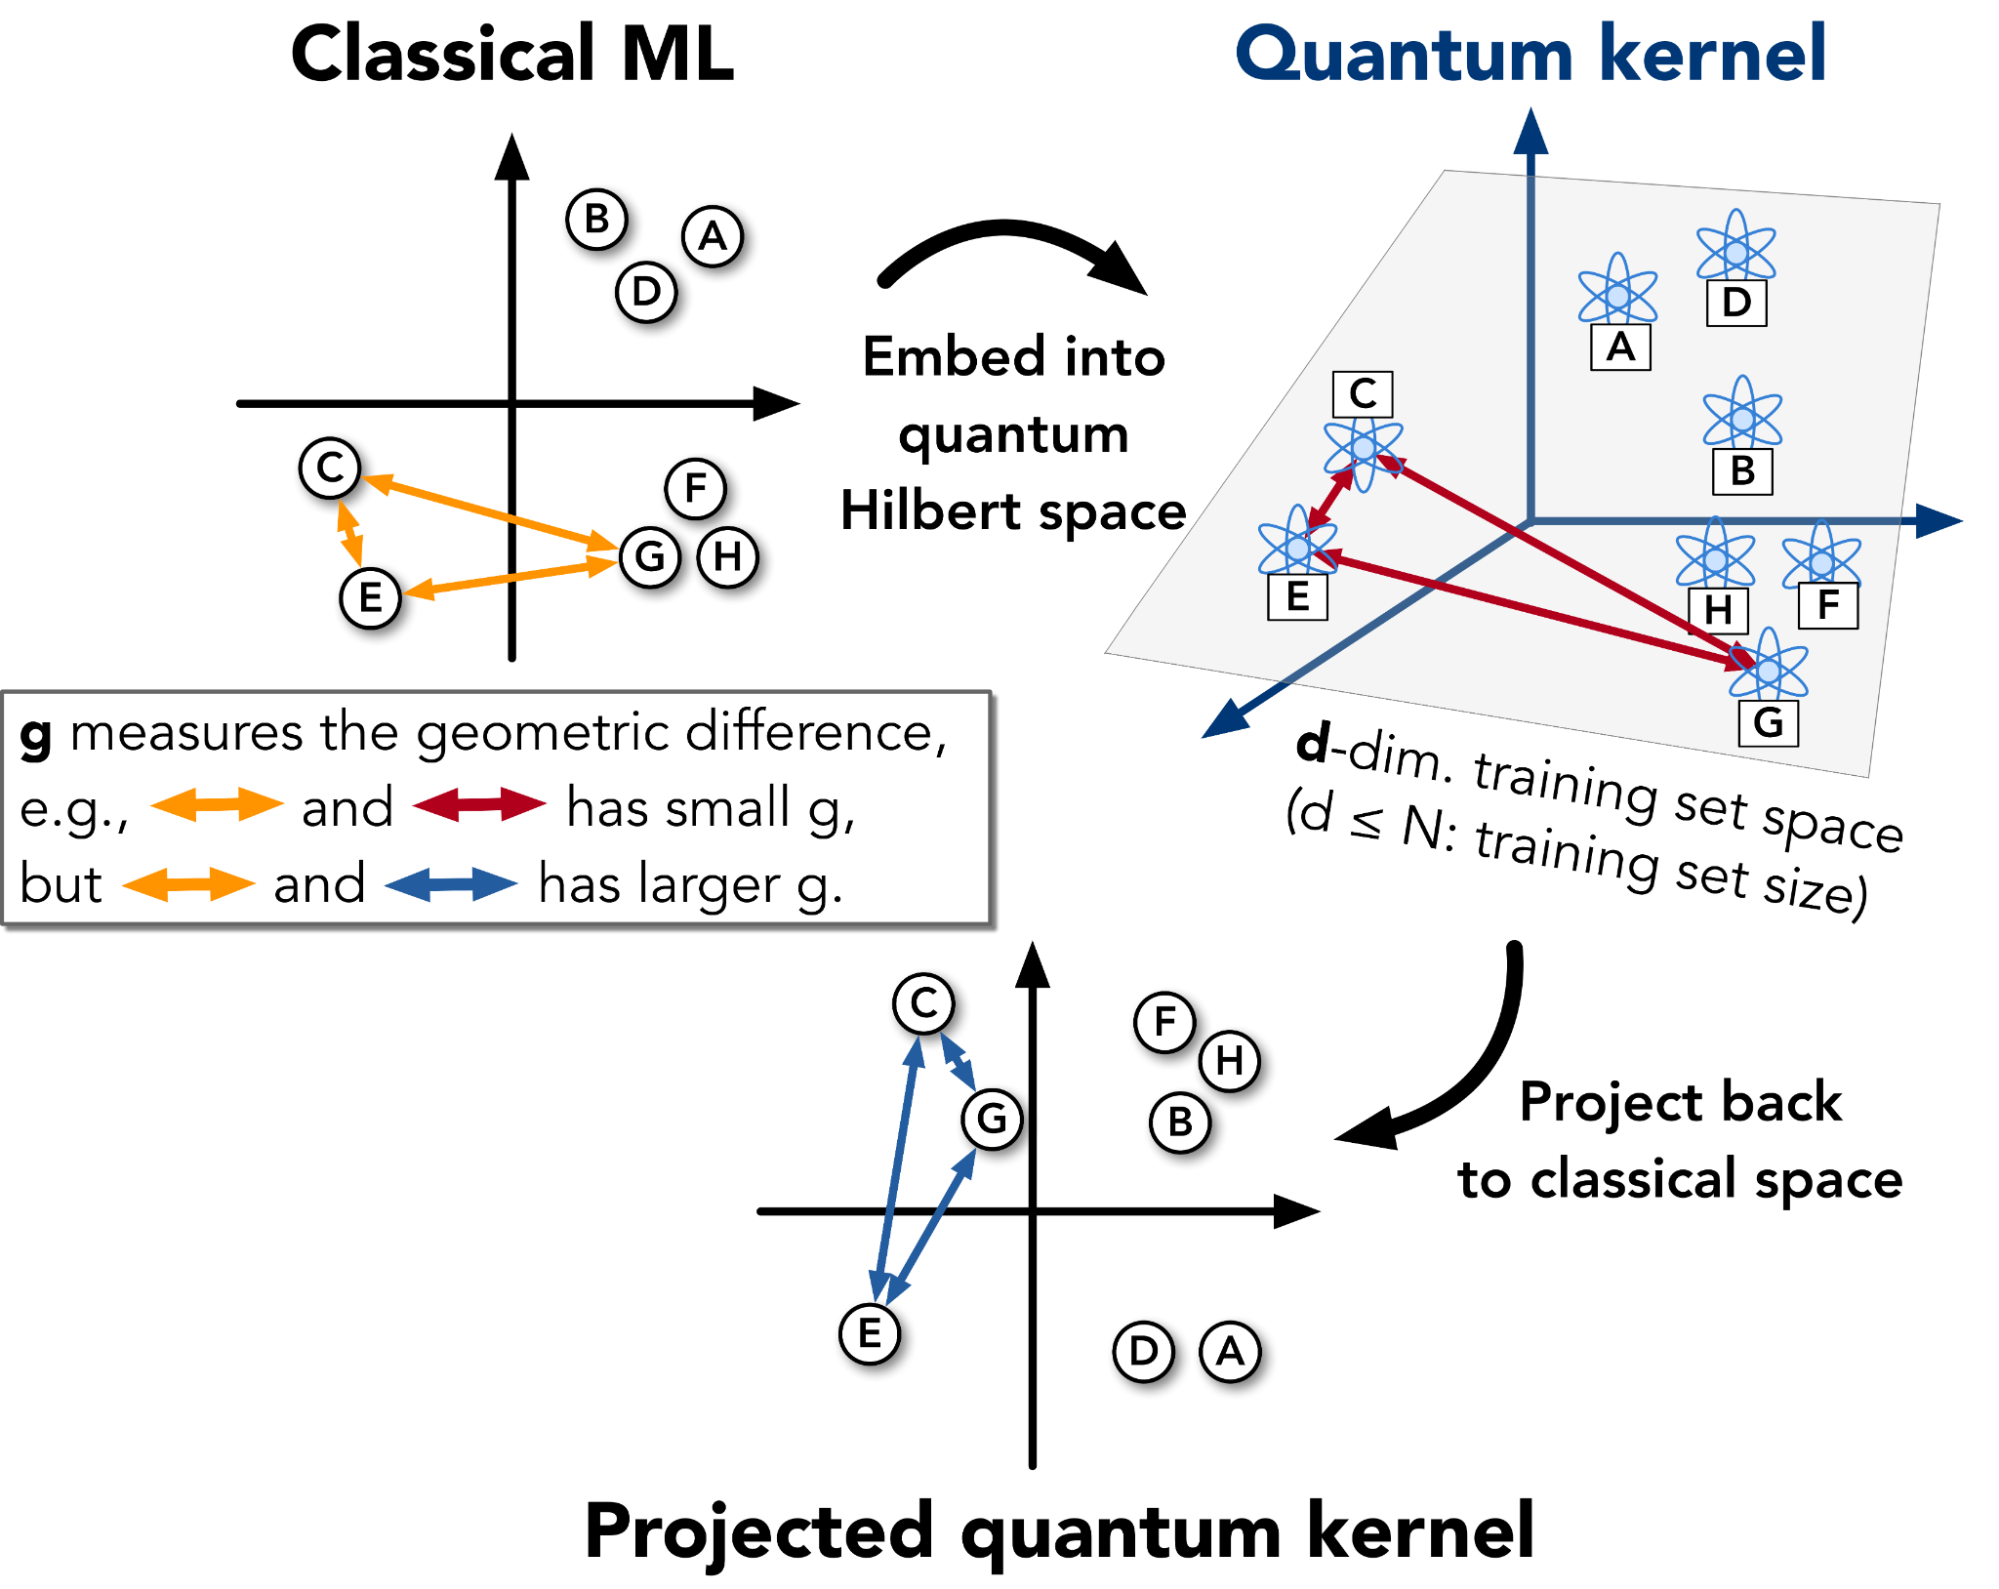
\includegraphics[width=0.8\textwidth]{QuantumKernel.png}
\caption{Projection of classical machine learning methods into a quantum hilbert space. Where $g$ is a geometric quantity which quantifies the potential for quantum advantage.\cite{mcclean_huang_2021}}
\end{figure}

I want to dissect two different approaches to quantum machine learning done in recent years. One such approach is quantum neural networks (QNN), which uses a quantum circuit to create a neural network similar to its classical counterpart. The other is quantum linear regression (QLR) which takes advantage of various algorithms we've learned throughout the course - such as the HHL algorithm, quantum fourier transform, and phase estimation.
\subsection*{Quantum Neural Networks (QNN)}
In 2018 Google and MIT demonstrated the creation of a small quantum neural network on a quantum simulator. \cite{farhi2018classification} This algorithm was also designed with near-team quantum computers in mind, being able to run on super conducting chips once their error rate and fidelity is further improved.

\begin{figure}[h]
\centering
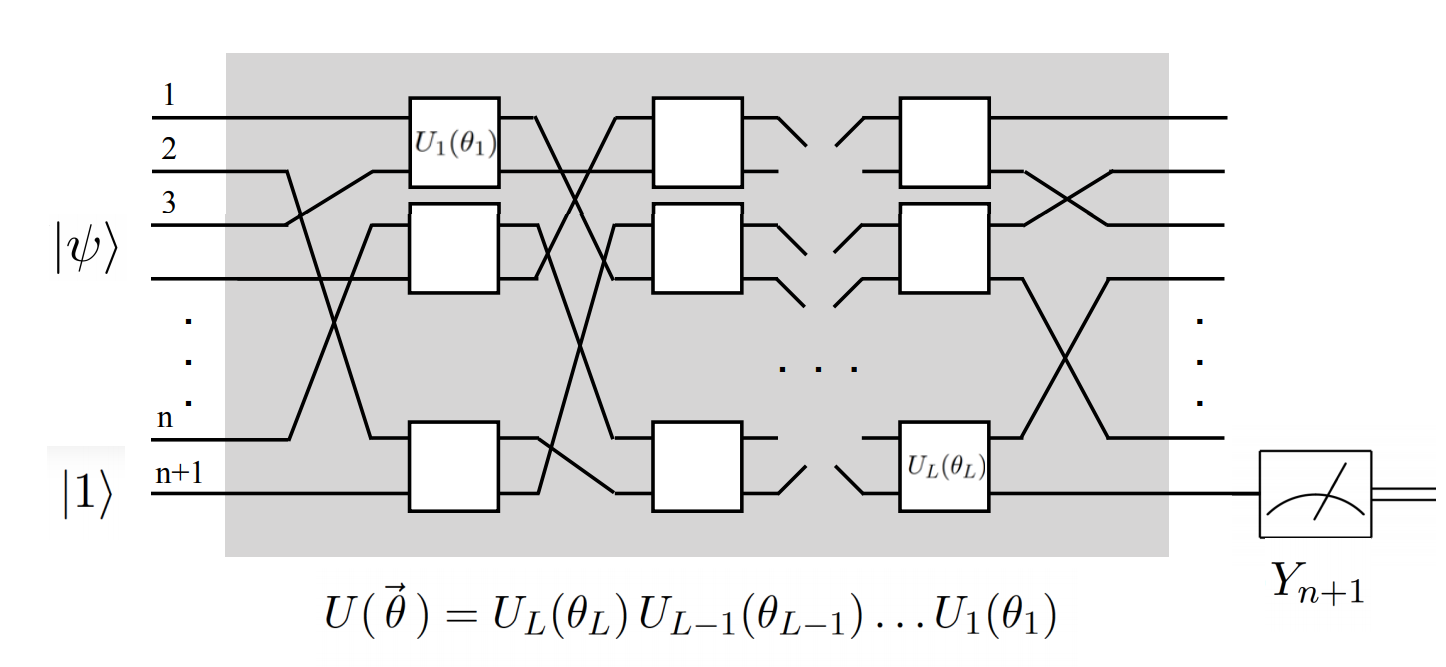
\includegraphics[width=0.8\textwidth]{QNN_Algo.png}
\caption{Quantum neural network circuit built from a set of $L$ unitaries which depend on some continuous set of parameters $\theta$.}
\end{figure}

This QNN algorithm operates on N+1 qubits of input, where a single additional qubit is used to measure output. It creates a neural network from a basic set of $L$ unitary gates which depend on some continuous set of parameters $\theta$. The goal is to have the measured output from a prepared state $|\psi\rangle$ match a given label $l(z)$. The output is measured in the Pauli Y basis (denoted as $Y_{n+1}$), yeilding a value of $+1$ or $-1$. A loss function can be generated from the measured results in the form:
\begin{equation}
    \text{loss} (\theta, z) = 1 - l(z) \langle z, 1| U^\dagger(\theta)Y_{n+1} U(\theta) |z, 1\rangle
\end{equation}

Different values of thetas can be sampled from neighboring unitaries and the loss function can be minimized. This process is known as gradient descent. The algorithm is summarized in the figure above.

\subsection*{Quantum Linear Regression (QLR)}
Quantum linear regression proves to provide a polynomial speedup over its classical counterpart. This was achieved by a 2017 paper by Guoming Wang from University of Maryland. \cite{Wang_2017} The algorithm is based mostly on the use of the HHL algorithm, which we learned about in class. This is due to the fact that linear regression relies on solving a system of linear equations to best fit the input data. \\
The HHL algorithm works for a linear system in the form of $Ax = b$, where $A$ is a Hermitian matrix, $x$ is a vector of unknowns, and $b$ is the output state we're trying to solve for. Since $A$ is Hermitian, it can be decomposed into a sum of its eigenvalues and eigenvectors like so:
\begin{equation}
    A = \sum_{i=1}^n \lambda_i |v_i\rangle \langle v_i|
\end{equation} 
Since $A$ is also invertible, we can write $A^{-1}$ as:
\begin{equation}
    A^{-1} = \sum_{i=1}^n \frac{1}{\lambda_i} |v_i\rangle \langle v_i|
\end{equation}
$|b\rangle$ can be written as a linear combination of the eigenvectors of $A$:
\begin{equation}
    |b\rangle = \sum_{i=1}^n \alpha_i |v_i\rangle
\end{equation}
Therefore we can simply solve for $|x\rangle$ by multiplying $A^{-1}$ by $|b\rangle$:
\begin{equation}
    |x\rangle = \sum_{i=1}^n \frac{\langle u_i | b \rangle }{\lambda_i} |v_i\rangle
\end{equation}
Thus, we can construct a quantum circuit that solves for $|x\rangle$ by first preparing the state $|b\rangle$ and extracting its eigenvalues with the quantum phase estimation algorithm; This will encode the eigenvalues into a quantum state. Applying eigenvalue inversion gives us the inverted eigenvalues, which can be converted back into amplitudes for measurement using an inverted form of the phase estimation algorithm. This can be done exponentially faster than a classical algorithm and provides a polynomial speedup for QLR.\cite{palsberg_2022}\cite{Wang_2017} The HHL algorithm is summarized in the figure below.
\begin{figure}[h]
\centering
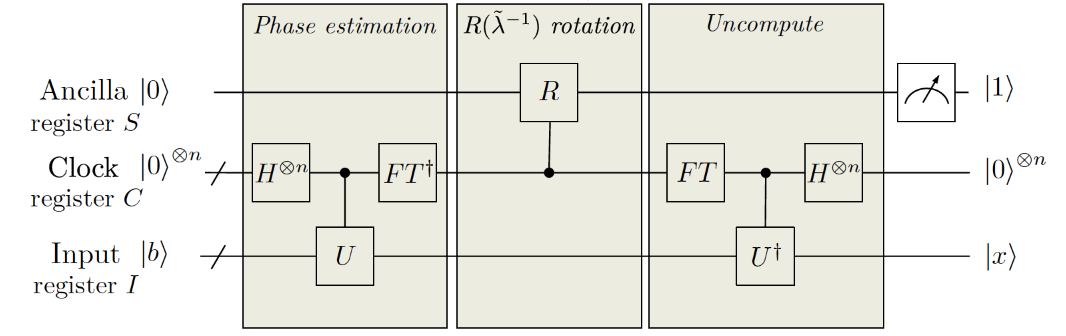
\includegraphics[width=0.9\textwidth]{HHL_Algo.png}
\caption{HHL algorithm for solving a linear system of equations. \cite{palsberg_2022}}
\end{figure}

\subsection*{Quantum Annealing}
\begin{figure}[h]
\centering
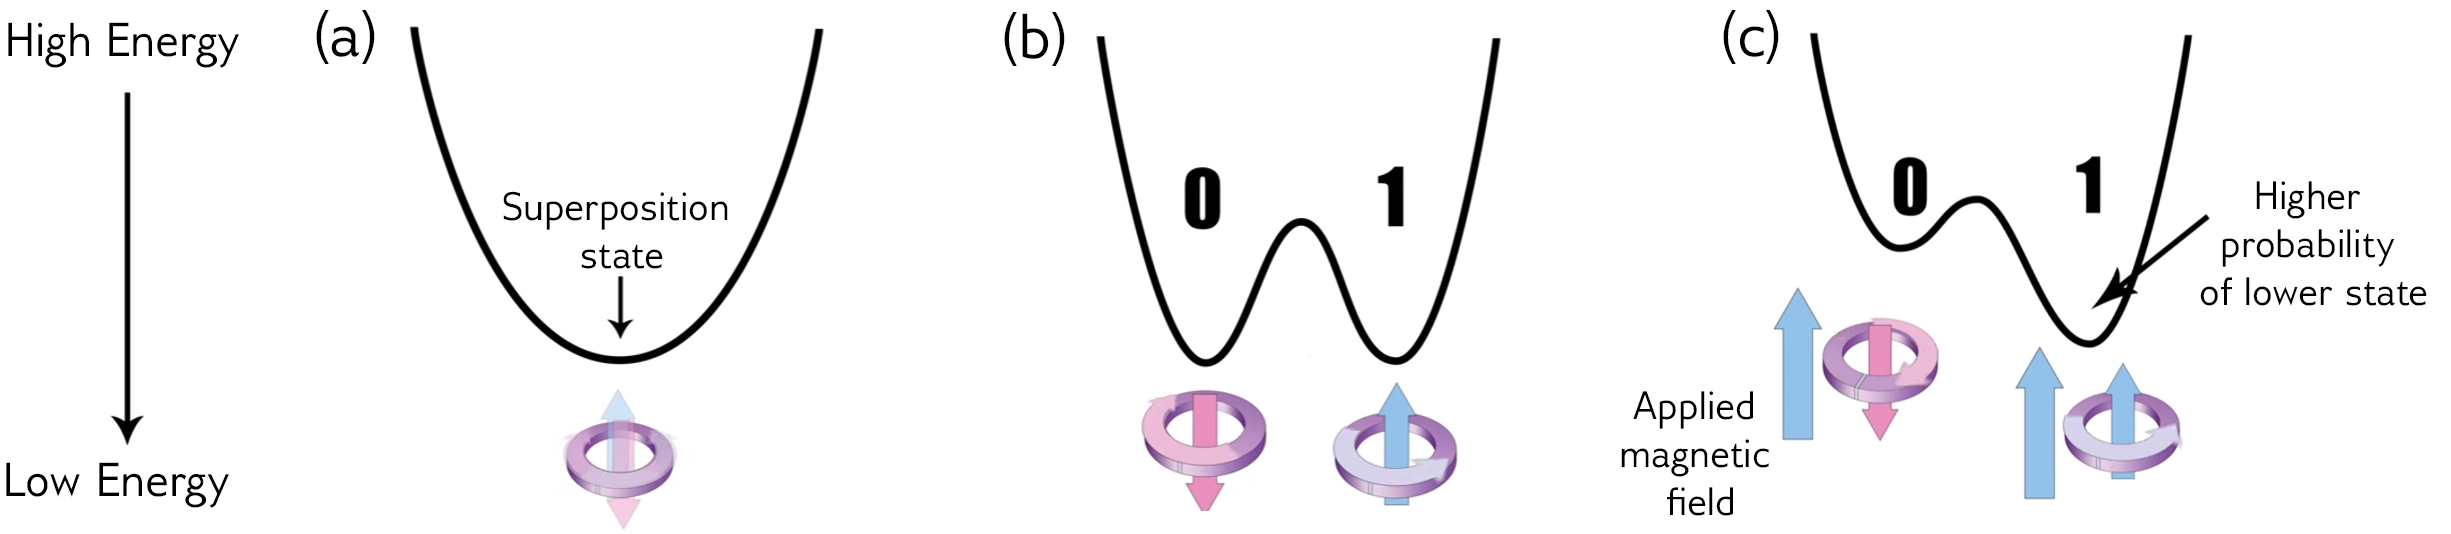
\includegraphics[width=1\textwidth]{QuantumAnnealing.png}
\caption{Quantum }
\end{figure}
An additional approach to quantum machine learning is quantum annealing. Quantum annealing takes advantage of the fact that quantum systems follow the laws of thermodynamics. Overtime, a quantum system will decay into its lowest state of energy - known as the ground state. This means that the global minima of a function can be mapped to the ground state of a quantum system. This is done by encoding the function as a Hamiltonian and then running the system through a quantum annealer. The company D-Wave Systems has worked to develop quantum annealers that can be used to do do linear regression and solve specific optimization problems.\cite{adachi_henderson_2021} \cite{date_potok_2021}


% OUTLINE:\\
% - Summarize quantum algorithms
% - Go over basics of how they work and discuss the algorithms they include (especially HHL and the ones we've used in class)
% - Choose a couple quantum algorithms and discuss how they work
% - Discuss how they imrpove upon classical algorithms
% - Discuss how they are used today

% % - Basic linear algebra subroutine (BLAS) which includes fourier transforms, solving linear equations, and eignvalue decomposition, are speedupable by quantum algorithms.
% - Quantum annealing


\section*{Advantages of QML}
\subsection*{Computational Complexity}
We've seen that quantum approaches to machine learning are able to provide polynomial and exponential runtime speedups to the classical algorithms of neural networks and linear regression. As mentioned earlier, the HHL algorithm is an example of this computational speedup. Quantum systems naturally work in hilbert spaces decomposable by a set of eigenvalues and eigenvectors. Therefore, we can take advantage of this fact to quickly estimate the solution of a system of linear equations. Since linear regression relies heavily on solving a system of linear equations, the HHL algorithm proves very promising for quantum linear regression.

\subsection*{Data Efficiency}
Machine learning needs a significant sample of training data in order to perform optimally. Even if a machine learning algorithm runs quickly, it may still take a while to achieve good results due to the fact that it needs a lot of training data. QML has the ability to perform more efficiently with less data than its classical counterpart. This is key in machine learning, as the more data you have, the more accurate your model typically will be. This suggests that with scale, quantum machine learning could possibly outperform classical machine learning purely due to the fact that it needs to process less data to achieve the comparable results. \cite{Huang2021}

\section*{Disadvantages of QML}
\subsection*{HHL can only be used for specific problems}
As we noticed in class, the HHL algorithm comes with quite a few limitations. It requires that the eigenvalues of the matrix to be known ahead of time in order to preform proper eigenvalue decomposition. It also requires that the matrix be Hermitian, which is not always the case. HHL also cannot output negative solutions. This means that additional time must be spent classically to find which parts of the output vector are positive and negative.
\subsection*{Hardware limitations}
Quantum computers are still in their infancy; they are still noisy and error-prone. This of course means that quantum algorithms are not nearly as reliable as their classical counterparts when ran on a quantum system. QML algorithms can be run with complete accuracy on quantum simulators, however, simulators still need lots of classical processing power and can only scale to a handful of qubits before they run out of memory. It will probably be awhile before we see quantum computers that can run QML algorithms with the same accuracy as classical computers.\\
Additionally, some methods of QML require the use of qRAM, which has not yet been developed. QRAM allows for loading in of additional quantum states later on into an a circuit. This is particularly useful for dealing with large amounts of data, which QNN and QLR both require.

\section*{Conclusion}
Quantum neural networks and quantum linear regression are two promising approaches to QML. They both provide polynomial speedups over their classical counterparts. Quantum annealing is another approach to QML that is still in its infancy. It is able to provide exponential speedups over classical algorithms, but it is still limited by the fact that it can only be used for specific problems. In general, there are quite a few limitations to QML, but it is still a very promising field of research. As quantum computers become more reliable and more qubits are added to quantum systems, we will see more and more applications of QML in the real world.

\bibliographystyle{plain} % We choose the "plain" reference style
\bibliography{refs} % Entries are in the refs.bib file

\end{document}